\section{Story Maintenance}

Managing Stories
\newline
Stories for a project can easily be added, deleted and updated using murcS. To begin select 'Story' in the Display Choice picker (circled below)

\begin{figure}[H]
\centering
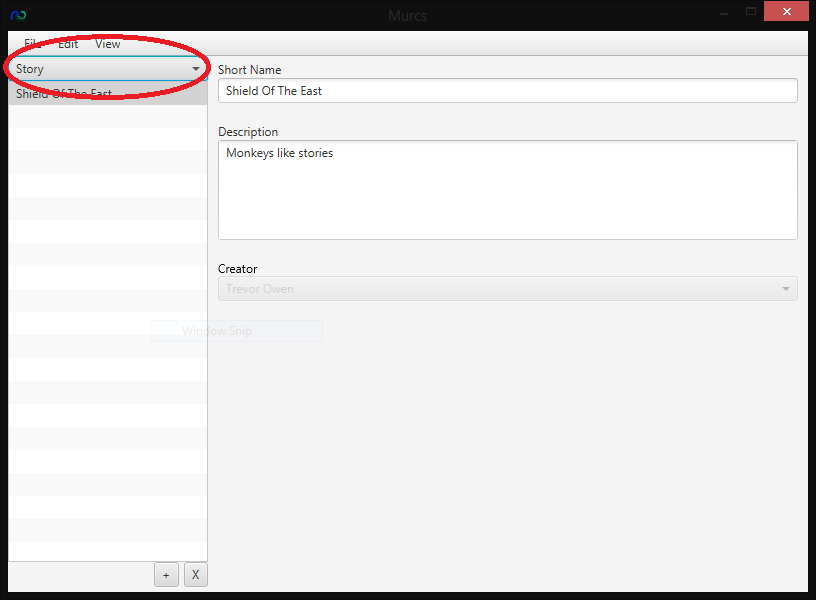
\includegraphics[width=\textwidth]{images/screenshots/stories1.PNG}
\caption{The Display Choice Picker}
\label{fig:new_project}
\end{figure}

Creating Stories
Stories can be created in two different ways, by clicking the add button (circled in red in the image below) or by navigating File-->New-->Story.

\begin{figure}[H]
\centering
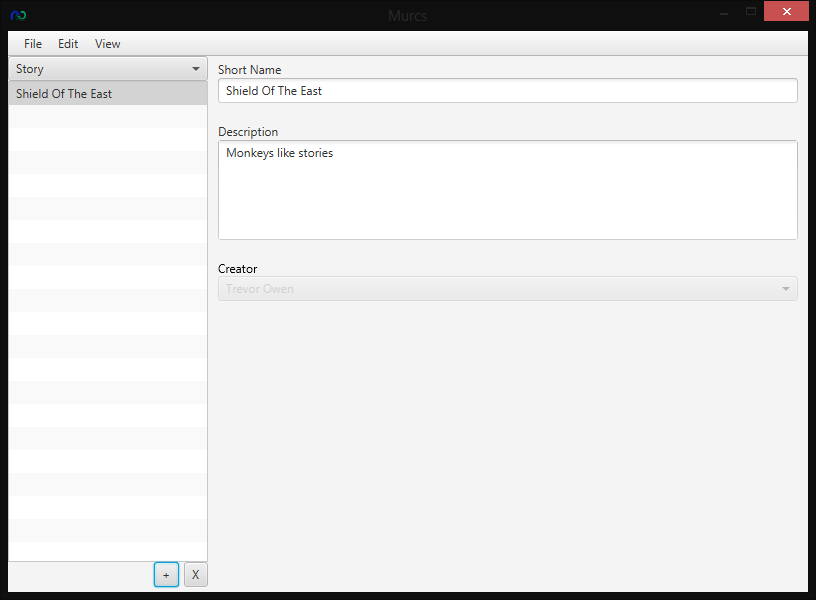
\includegraphics[width=\textwidth]{images/screenshots/stories2.PNG}
\caption{The Story Creation Dialog}
\label{fig:new_project}
\end{figure}

Whichever way you chose to create your story you will have been greeted with the following 'Story Creation Dialog' (pictured below). When creating a story you can specify a number of different fields. 

Name:
This is the name of your story. It must not be empty and must be unique, but you can change it later. This will show up in the display list, so make it recognizable!

Description:
To make life easier for your team it is helpful to know what a story is about. This is where the description field comes in. The description can be anything you like, but is most useful if it describes the story. You can change the description at any point.

Creator:
This field stores the original creator of the story. It cannot be changed after the project has been created, so make sure you get it right first time.

Updating
To update an existing story, simply select it from the display list. In the below picture we are editing the story known as 'A Story.' Note how the creator field is greyed out and cannot be changed.

\begin{figure}[H]
\centering
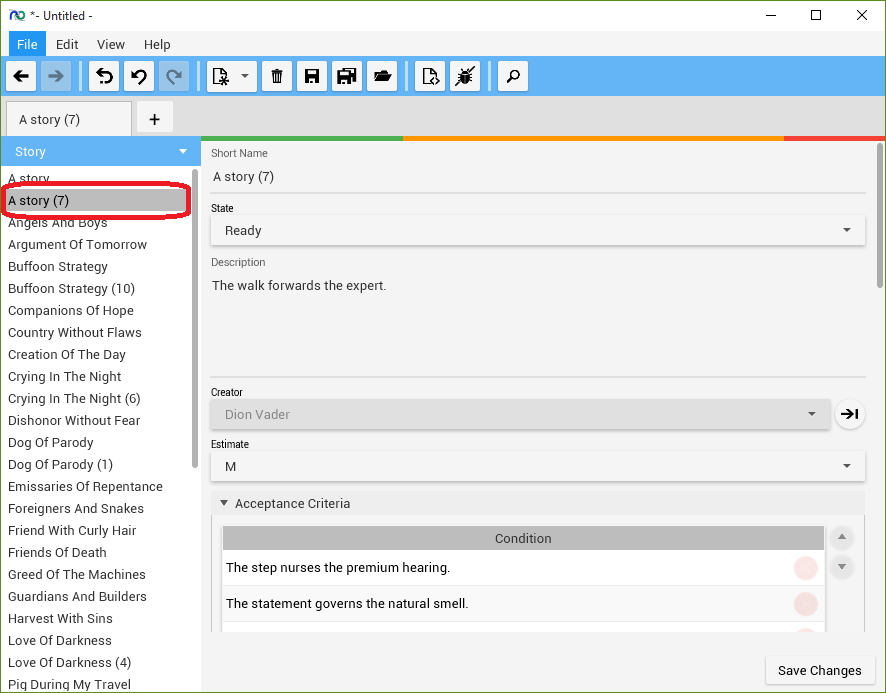
\includegraphics[width=\textwidth]{images/screenshots/stories4.PNG}
\caption{The Editing Pane}
\label{fig:new_project}
\end{figure}

Story State\newline
The Story State property (circled below) defines the state a story is currently in. If you try to change this but the state is not supported an error message will be displayed at the bottom of the editor. \newline

Requirements\newline
None: No requirements\newline
Ready: Story is in a backlog, story has at least one AC and story is estimated

\begin{figure}[H]
\centering
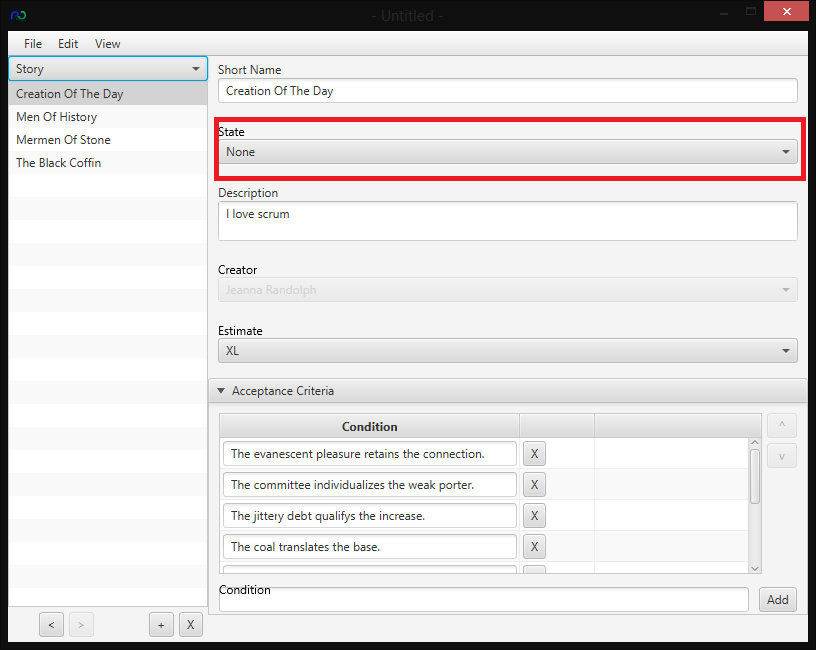
\includegraphics[width=\textwidth]{images/screenshots/Readiness1.PNG}
\caption{The Story State Property}
\label{fig:new_project}
\end{figure}

Estimating\newline
To create an estimate for a story, your story must first be part of a backlog and have at least one Acceptance Condition (see below). The scale you estimate on depends on the scale specified in the backlog that this story is attached to. If you change this type on the backlog the program will do it's best to work out what the equivalent is on the new scale.

\begin{figure}[H]
\centering
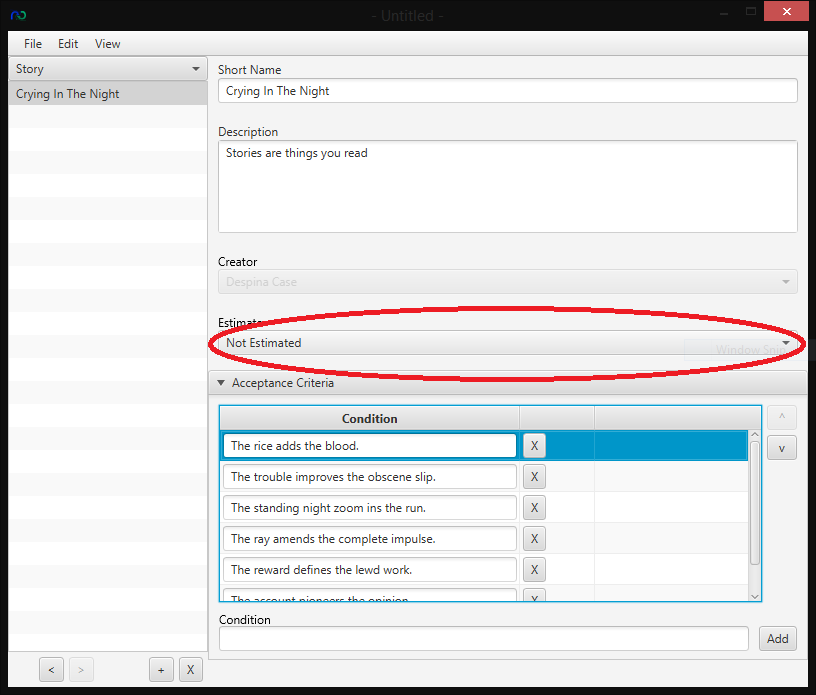
\includegraphics[width=\textwidth]{images/screenshots/Estimate1.PNG}
\caption{The Estimate Property}
\label{fig:new_project}
\end{figure}

Acceptance Criteria (ACs)\newline
A story can have any number of acceptance criteria. However, you should note that there are some things you cannot do to a story if it does not have an ACs (such as estimating that story or changing its state to ready). Acceptance criteria can be managed using "Acceptance Criteria" pane (marked below) while editing a story.

\begin{figure}[H]
\centering
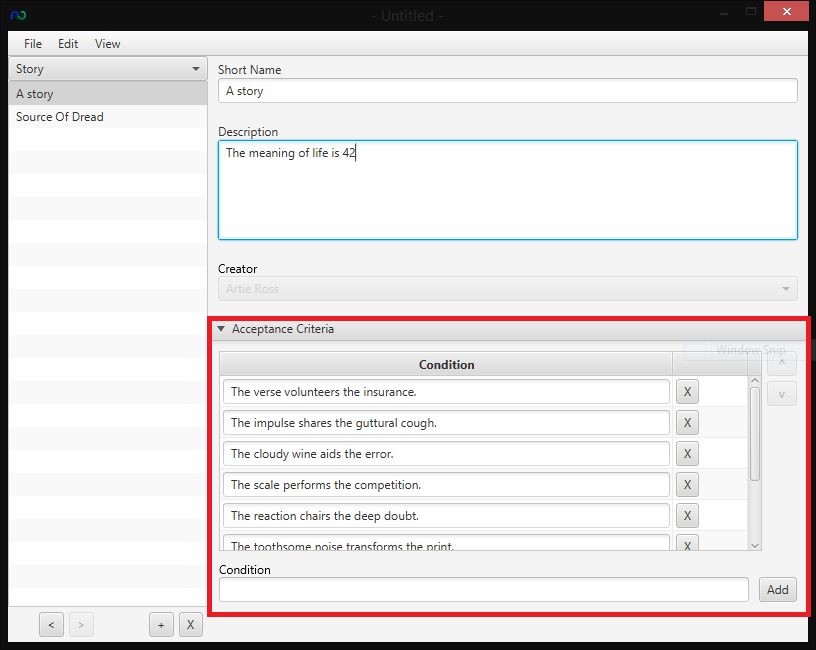
\includegraphics[width=\textwidth]{images/screenshots/AcceptanceCriteria1.PNG}
\caption{The Acceptance Criteria Pane}
\label{fig:new_project}
\end{figure}

You can create a new Acceptance Condition by typing in the "Add Condition" text field (marked below) and pressing the add button. New acceptance conditions will be added at the end of the list by default.

\begin{figure}[H]
\centering
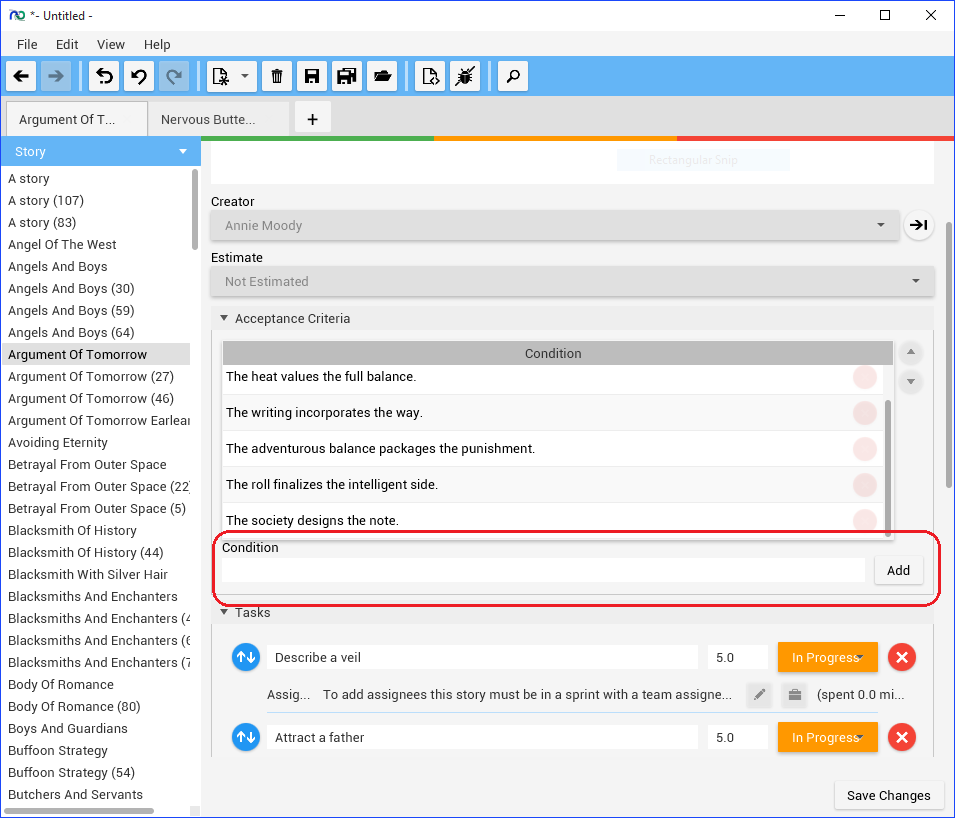
\includegraphics[width=\textwidth]{images/screenshots/AcceptanceCriteria2.PNG}
\caption{The Add Condition Field}
\label{fig:new_project}
\end{figure}

You can edit the condition on an AC by simply typing in the relevant text field. Your changes will be saved automatically, when you click away. Similarly, you can delete a condition using the 'X' button in the second column of the table.
\newline\newline

Acceptance Conditions can also be moved up and down in the list, depending on their priority. To do this, use the up and down arrows (marked below). A condition cannot be moved up from the top of the list or down from the bottom.

\begin{figure}[H]
\centering
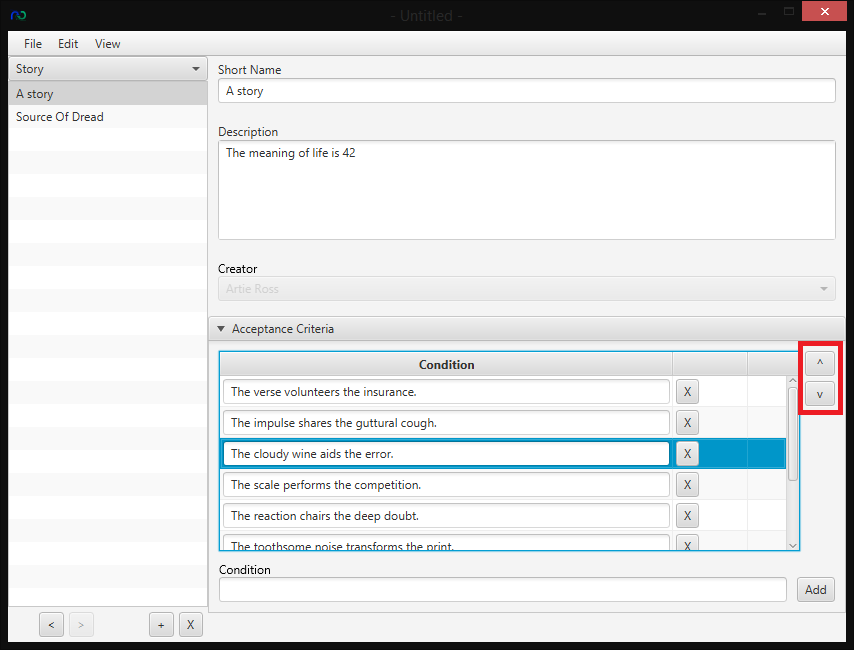
\includegraphics[width=\textwidth]{images/screenshots/AcceptanceCriteria3.PNG}
\caption{The Priority Buttons}
\label{fig:new_project}
\end{figure}

Dependencies\newline
You can manage dependencies in the dependencies area of the story pane. To add a story as a dependency, simply start typing its name or select it from the list box provided. Dependencies must be transitive (they cannot cause dependency cycles). Attempting to add a dependency that will cause a cycle will result in an error.\newline
Removing a dependency is done in the same way as for Acceptance Criteria. Pressing the 'X' button on the right hand side of each dependency will remove it from the story.\newline
Depth of a dependency, as indicated to the left side of the 'X' button, describes the maximum number of dependencies that the dependency itself transitively depends on.\newline\newline

Deletion\newline
To delete a story, simply press the delete button (the bin in the tooblar). You will be greeted with a confirmation dialog that will notify you of all the places the story is used. From this dialog you can go through with the deletion or cancel if you change your mind. For more information, see the 'Element Deletion' section of this guide.

\begin{figure}[H]
\centering
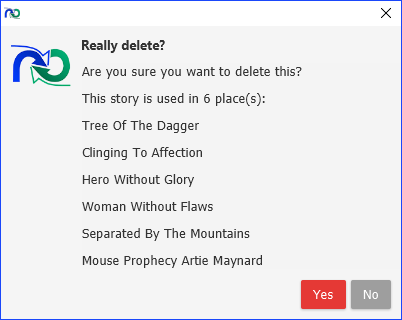
\includegraphics[width=\textwidth]{images/screenshots/stories5.PNG}
\caption{Deleting a Story}
\label{fig:new_project}
\end{figure}